% mnras_template.tex 
%
% LaTeX template for creating an MNRAS paper
%
% v3.2 released 20 July 2023
% (version numbers match those of mnras.cls)
%
% Copyright (C) Royal Astronomical Society 2015
% Authors:
% Keith T. Smith (Royal Astronomical Society)

% Change log
%
% v3.2 July 2023
%	Updated guidance on use of amssymb package
% v3.0 May 2015
%    Renamed to match the new package name
%    Version number matches mnras.cls
%    A few minor tweaks to wording
% v1.0 September 2013
%    Beta testing only - never publicly released
%    First version: a simple (ish) template for creating an MNRAS paper

%%%%%%%%%%%%%%%%%%%%%%%%%%%%%%%%%%%%%%%%%%%%%%%%%%
% Basic setup. Most papers should leave these options alone.
\documentclass[fleqn, usenatbib]{mnras}

% MNRAS is set in Times font. If you don't have this installed (most LaTeX
% installations will be fine) or prefer the old Computer Modern fonts, comment
% out the following line
\usepackage{newtxtext, newtxmath}
% Depending on your LaTeX fonts installation, you might get better results with one of these:
%\usepackage{mathptmx}
%\usepackage{txfonts}

% Use vector fonts, so it zooms properly in on-screen viewing software
% Don't change these lines unless you know what you are doing
\usepackage[T1]{fontenc}

% Allow "Thomas van Noord" and "Simon de Laguarde" and alike to be sorted by "N" and "L" etc. in the bibliography.
% Write the name in the bibliography as "\VAN{Noord}{Van}{van} Noord, Thomas"
\DeclareRobustCommand{\VAN}[3]{#2}
\let\VANthebibliography\thebibliography
\def\thebibliography{\DeclareRobustCommand{\VAN}[3]{##3}\VANthebibliography}


%%%%% AUTHORS - PLACE YOUR OWN PACKAGES HERE %%%%%

% Only include extra packages if you really need them. Avoid using amssymb if newtxmath is enabled, as these packages can cause conflicts. newtxmatch covers the same math symbols while producing a consistent Times New Roman font. Common packages are:
\usepackage{graphicx}	% Including figure files
\usepackage{amsmath}	% Advanced maths commands
\usepackage[acronym]{glossaries} % for acronyms
\usepackage{physics} % Physics symbols
\usepackage[section]{placeins} % Place figures and tables inside the section they are defined in

% \usepackage{showlabels} % To show equations labels on the PDF. Comment at the end

%%%%%%%%%%%%%%%%%%%%%%%%%%%%%%%%%%%%%%%%%%%%%%%%%%

%%%%% AUTHORS - PLACE YOUR OWN COMMANDS HERE %%%%%

\glsdisablehyper % Disable hyperlinks on acronyms
\newacronym{ssfr}{sSFR}{specific star formation rate}
\newacronym{ms}{MS}{main sequence}
\newacronym{sf}{SF}{star formation}
\newacronym{dm}{DM}{dark matter}
\newacronym{sdss}{SDSS}{Sloan Digital Sky Survey}
\newacronym{cigale}{CIGALE}{Code Investigating GALaxy Emission}
\newacronym{sfr}{SFR}{star formation rate}

%%%%%%%%%%%%%%%%%%%%%%%%%%%%%%%%%%%%%%%%%%%%%%%%%%

%%%%%%%%%%%%%%%%%%% TITLE PAGE %%%%%%%%%%%%%%%%%%%

% Title of the paper, and the short title which is used in the headers.
% Keep the title short and informative.
\title[Laboratory of Data Analysis]{Laboratory of Data Analysis - The specific star formation rate populations}

% The list of authors, and the short list which is used in the headers.
% If you need two or more lines of authors, add an extra line using \newauthor
\author[F. Leto di Priolo]{
Federico Leto di Priolo}

% These dates will be filled out by the publisher
\date{July 2024}

% Enter the current year, for the copyright statements etc.
\pubyear{2024}

% Don't change these lines
\begin{document}

\maketitle

% Abstract of the paper
\begin{abstract}
	Using simple models and empirical laws, we present some possible descriptions of the two galaxies populations we observe: star-forming galaxies and passive galaxies. We focus on the \acrfull{ssfr} vs stellar mass relation and on the physical process leading to \acrshort{ssfr} quenching for a fraction of the massive galaxies. We work using photometry data from the \acrfull{sdss} processed by the \acrfull{cigale} package. Our results rely on three main models: the Open-box, the Closed-box and the numerically evolved model of a galaxy. The Open-box solution is a fairly good representation of our data for star-forming galaxies, while the Closed-box model roughly captures the properties of the \acrshort{ssfr} of passive galaxies. We believe that the numerical approach should be preferred over the others, even though our implementation suffers a relevant discrepancy in magnitude from our data. Ineffective gas cooling due to galaxies haloes growth plays a key role in determining the transition from the star-forming regime to the passive one. Our estimate of the stellar mass threshold between the two regimes seems reasonable for our simple description. The non-numerical approaches might be valid as well, but a deeper refinement of such models is necessary.
\end{abstract}

% Select between one and six entries from the list of approved keywords.
% Don't make up new ones.
\begin{keywords}
	galaxies: evolution -- galaxies: haloes -- galaxies: star formation
\end{keywords}

%%%%%%%%%%%%%%%%%%%%%%%%%%%%%%%%%%%%%%%%%%%%%%%%%%

%%%%%%%%%%%%%%%%% BODY OF PAPER %%%%%%%%%%%%%%%%%%

\section{Introduction}

Observations highlight a strong bimodality in the galaxy population: the \acrlong{ssfr} is higher for lower mass galaxies and drops rapidly after a certain mass threshold. We can identify a \acrfull{ms} of blue galaxies forming stars with nearly constant \acrshort{ssfr}, and a region of red passive galaxies at high stellar masses. Our focus is on the \textbf{physical processes} that determine the \textbf{quenching of \acrshort{ssfr}} for a fraction of the massive galaxies. The \acrfull{sf} in galaxies is tuned by many different phenomena; we used some simple models to try to explain the observed behavior of the \acrshort{ssfr} vs. mass relation. We tried to understand which models better describe the two populations, which assumptions could be relaxed, and which parameters mostly change the results when modified. This helps to understand which physical processes are more relevant for the \acrshort{sf} in the two galaxy populations. Specifically, we want to answer the following questions: \textit{Can the two populations be described independently?} \textit{What determines the transition from the star-forming regime to the passive one?} \textit{Does redshift play a crucial role in the description of the two populations?}

Two main approaches have been used:
\begin{itemize}
	\item Time-independent models capturing the average behavior of the \acrshort{ssfr};
	\item Time-evolving models that track the \acrlong{sf} up to the present time.
\end{itemize}
In both cases, one of the key elements is the transition from the star forming regime to the passive regime. This is closely related to the \acrfull{dm} haloes of galaxies, which are connected to the cooling rate of the free gas.

We will first describe the general framework we worked in and then discuss the development of each model. Finally, we will show how the two types of models perform compared with the data and talk about possible improvements. The main instruments of this work are the \acrlong{sdss} catalogue, the \acrshort{cigale} package, and some simple Python scripts for the development and testing of the models.

\section{Framework}

There, we will talk about the \acrshort{sdss} catalogue, the \acrshort{cigale} package, and the general equation regulating the \acrfull{sfr} in galaxies, from which we started for the development of our models.

\subsection{\acrshort{sdss} and \acrshort{cigale}}

The \acrshort{sdss} provides the most complete three-dimensional map of the universe we have access to. It offers multi-epoch optical and IR spectroscopy across the entire sky for millions of astronomical objects. In particular, we used photometric data of 92482 galaxies at low redshift \(z \simeq 0.05\). To infer physical properties of galaxies from the data, we then used the \acrshort{cigale} package.

\acrshort{cigale} has been developed to study the evolution of galaxies by comparing modeled galaxy spectral energy distributions to observed ones. Galaxies' physical properties such as stellar mass, \acrshort{sfr}, and age are derived with a maximum likelihood algorithm that tests every possible model for each galaxy. The model set is determined by a discrete parameters grid given as input. \acrshort{cigale} also provides a wide range of models for star formation histories, stellar populations, dust attenuation, and emission.

We used the results obtained from \acrshort{cigale} and the \acrshort{sdss} catalogue to analyze galaxy properties and develop our models.

\subsection{Star formation equation}

The \acrlong{sfr} quantifies the amount of mass converted into stars per unit time. This depends mainly on the available amount of gas and on the environment the galaxy lives in. We need to understand how the environment influences the conversion of gas into stars and vice versa.
We can then define the stellar mass as:
\begin{equation} \label{eq:stellar_mass}
	M_{\star} = \int_{t_0}^t \dot{M}_\star(t')dt'
\end{equation}
where \(\dot{M}_{\star}\) is the \acrshort{sfr}, and \(t - t_0\) is the age of the galaxy.

We consider a galaxy within its dark halo and write down the differential equation expressing the conservation of gas mass:
\begin{equation} \label{eq:gas_conservation}
	\dot{M}_{\mathrm{gas}} = \dot{M}_{\mathrm{gas, in}} - (1 - R) \dot{M}_{\star} - \dot{M}_{\mathrm{gas, out}}
\end{equation}
where \(\dot{M}_{\mathrm{gas, in}}\) and \(\dot{M}_{\mathrm{gas, out}}\) are the gas accretion and outflow rates, and \(R\) is the recycled fraction of gas due to supernovae explosions and stellar winds. We will start from this equation to develop both the time-independent and the time evolving models.

To get a solution for Equation \ref{eq:gas_conservation}, we will make use of an empirical relation from \citet{Kennicutt1997}:
\begin{equation} \label{eq:kennicutt}
	\dot{M}_{\star} = \frac{\epsilon}{t_{\mathrm{dyn}}} M_{\mathrm{gas}}
\end{equation}
which means that, on average, every free-fall time, a fraction \(\epsilon\) of the available gas mass is converted into stars. Typically, this fraction is around \(1\% - 2\%\). For disk-like star-forming galaxies the dynamical time can be written as:
\begin{equation} \label{eq:t_dyn}
	t_{\mathrm{dyn}} = 2 \times 10^7\ \mathrm{yr}\ \qty(\frac{R_{1/2}}{4\ \mathrm{kpc}}) \qty(\frac{V_c}{200\ \mathrm{km\ s^{-1}}})^{-1}
\end{equation}
where \(R_{1/2}\) is the half-light radius, and \(V_c\) is the circular velocity of the disk. However, since we don't have direct access to measurements of those quantities, for simplicity, we will use fixed values around \(2 \times 10^7\ \mathrm{yr}\), neglecting its variability.

\subsection{Gas accretion and outflow}

Before diving into the models, let's talk about \(\dot{M}_{\mathrm{gas, in}}\) and \(\dot{M}_{\mathrm{gas, out}}\) in equation \ref{eq:gas_conservation}. \(\dot{M}_{\mathrm{gas, in}}\) is the gas accretion rate into the galaxy; this term is required observationally. For the gas to \textit{fall} from the outer halo into the galaxy, we need it not to be in hydrostatic equilibrium or, equivalently, the cooling time should be smaller than the dynamical time. In this context, we can write the gas inflow into the galaxy as a fraction of the matter accreting in the \acrshort{dm} halo:
\begin{equation} \label{eq:gas_in}
	\dot{M}_{\mathrm{gas, in}} = f_{\mathrm{b}} \xi \dot{M}_{\mathrm{H}}
\end{equation}
where \(f_{\mathrm{b}}\) is the cosmic baryonic fraction, \(\xi\) is a numerical factor typically less than or equal to \(1\), and \(\dot{M}_{\mathrm{H}}\) is the halo's mass accretion rate. For the baryonic fraction \(f_{\mathrm{b}}\) we used the value of \(0.15\). The simplest implementation is obtained by setting \(\xi\) to a step function equals to \(1\) when \(t_{\mathrm{cool}} < t_{\mathrm{dyn}}\) and \(0\) otherwise. This condition can be recast into one for the halo's mass: there is effective cooling if \(M_{\mathrm{H}}\) is inside a certain range \([M_{\mathrm{H, min}}, M_{\mathrm{H, max}}]\). For solar metallicities and redshift \(0\), this mass range can be roughly identified with \([10^9, 10^{12}]\ \mathrm{M_{\sun}}\) \citep{Mo2010}. From cosmological simulations, we also have an expression for the halo's mass accretion rate \citep{McBride2009}:
\begin{multline} \label{eq:halo_accretion}
	\expval{\dot{M}_{\mathrm{H}}} = 42\ \mathrm{M_{\sun}\ yr^{-1}}\ \qty(\frac{M_{\mathrm{H}}}{10^{12}\ \mathrm{M_{\sun}}})^{1.127}\\
	\times\ (1 + 1.17 z) \sqrt{\Omega_m (1 + z)^3 + \Omega_\Lambda}
\end{multline}
where \(\Omega_m\) and \(\Omega_\Lambda\) are the matter and dark energy content fractions of the universe, and we will assume them to be respectively \(0.3\) and \(0.7\). Finally, we can relate the halo's mass to the stellar mass of the galaxy using an empirical relation \citep{Moster2012}:
\begin{equation} \label{eq:m_star_vs_m_halo}
	\frac{M_{\star}}{M_{\mathrm{H}}} = 2 N \qty[\qty(\frac{M_{\mathrm{H}}}{M_1})^{-\beta} + \qty(\frac{M_{\mathrm{H}}}{M_1})^\gamma]^{-1}
\end{equation}
where \(N\), \(M_1\), \(\beta\) and \(\gamma\) are redshift-dependent numerical factors. See Appendix \ref{appendix:m_star_vs_m_halo_parameters} for details.

\(\dot{M}_{\mathrm{gas, out}}\) is the gas outflow from the galaxy. It should take into account every process that leads to the expulsion of gas from the galaxy reservoir. Some examples are supernovae explosions and ram pressure stripping, but in terms of \acrshort{sfr} quenching AGN feedback should also be considered in principle. For simplicity, we will assume that the main gas lost is due to type II supernovae and neglect other effects. Hence, we will write:
\begin{equation} \label{eq:gas_out}
	\dot{M}_{\mathrm{gas, out}} = \eta \dot{M}_{\star}
\end{equation}
where \(\eta\) is a numerical factor that regulates the strength of the supernova feedback.

With these ingredients in mind, we can now describe the models we developed to explain the observed \acrshort{ssfr} vs \(M_{\star}\) trend.

\section{Models}

We will describe three basic models and how we used them to get the final results. Specifically, we will discuss the following:
\begin{itemize}
	\item Open-box model;
	\item Closed-box model;
	\item Time-evolving numerical model.
\end{itemize}

\subsection{Open-box model}

In the Open-box model, the gas is free to enter and leave the galaxy. Let's substitute \eqref{eq:kennicutt} and \eqref{eq:gas_out} into \eqref{eq:gas_conservation}. We obtain:
\begin{equation} \label{eq:open_box}
	\dot{M}_{\mathrm{gas}} = \dot{M}_{\mathrm{gas, in}} - \hat{\epsilon} M_{\mathrm{gas}}
\end{equation}
where \(\hat{\epsilon} = (1 + \eta - R) \frac{\epsilon}{t_{\mathrm{dyn}}}\). We can distinguish two regimes: if \(\dot{M}_{\mathrm{gas, in}} \ll \hat{\epsilon} M_{\mathrm{gas}}\), \(M_{\mathrm{gas}}\) exponentially decreases; if \(\dot{M}_{\mathrm{gas, in}} \gg \hat{\epsilon} M_{\mathrm{gas}}\), \(M_{\mathrm{gas}}\) constantly increases. Both regimes come to an end when the underlying conditions stop being satisfied. When this happens, the gas reservoir approaches the equilibrium condition \(\dot{M}_{\mathrm{gas}} = 0\). We can then write the amount of gas at equilibrium as:
\begin{equation} \label{eq:open_box_gas_eq}
	M_{\mathrm{gas}}^{\mathrm{eq}} = \frac{\dot{M}_{\mathrm{gas, in}}}{1 + \eta - R} \frac{t_{\mathrm{dyn}}}{\epsilon}.
\end{equation}
If we now use \eqref{eq:kennicutt} and divide by the stellar mass we get an expression for the \acrlong{ssfr} at equilibrium:
\begin{equation} \label{eq:open_box_solution}
	\mathrm{sSFR}^{\mathrm{eq}} = \frac{\dot{M}_{\mathrm{gas, in}}}{M_{\star}} \frac{1}{1 + \eta - R}.
\end{equation}
In order to obtain a \acrshort{ssfr} vs \(M_{\star}\) relation, we also need to rewrite \(\dot{M}_{\mathrm{gas, in}}\) using \eqref{eq:gas_in}, \eqref{eq:halo_accretion} and \eqref{eq:m_star_vs_m_halo}, where unfortunately \eqref{eq:m_star_vs_m_halo} must be inverted numerically. Since we assumed a constant redshift \(z \simeq 0.05\) and we used a step function for \(\xi\) in Equation \ref{eq:gas_in}, \eqref{eq:open_box_solution} gives us a direct relation between the stellar mass and the \acrlong{ssfr} at equilibrium.

We will see that this model fits pretty well for galaxies on the \acrlong{ms}, but fails in describing the more massive, passive galaxies. We need then another model to account for those galaxies; the Closed-box model is a simple, possible choice to solve the problem.

\subsection{Closed-box model}

In the Closed-box model, there is neither accretion nor outflow of gas in the galaxy; therefore we set \(\dot{M}_{\mathrm{gas, in}} = \dot{M}_{\mathrm{gas, out}} = 0\) in Equation \ref{eq:gas_conservation}. Using \eqref{eq:kennicutt}, the solution of the resulting equation is an exponentially decreasing gas reservoir:
\begin{equation} \label{eq:closed_box_gas}
	M_{\mathrm{gas}}(t) = M_{\mathrm{gas}}(t_0) \exp(-b \Delta t)
\end{equation}
where \(b = (1 - R) \frac{\epsilon}{t_{\mathrm{dyn}}}\), \(\Delta t = t - t_0\), and \(M_{\mathrm{gas}}(t_0)\) is the gas mass at the beginning of the Closed-box regime. As has been done for the Open-box model, we can now use \eqref{eq:kennicutt} again and divide by the stellar mass to get an expression for the \acrshort{ssfr}:
\begin{equation} \label{eq:closed_box_solution}
	\mathrm{sSFR}(t) = \frac{M_{\mathrm{gas}}(t)}{M_{\star}(t)} \frac{\epsilon}{t_{\mathrm{dyn}}}.
\end{equation}
However, in this model, no equilibrium is reached and an explicit time dependence is present. Since our goal is to obtain a \acrshort{ssfr} vs \(M_{\star}\) relation, we need to convert the time dependence into a stellar mass one. In order to do it we can use \eqref{eq:halo_accretion} and \eqref{eq:m_star_vs_m_halo}, and make the assumption that every galaxy accretes its halo mass at a constant rate at every time. Doing so, we can rewrite the \(\Delta t = t - t_0\) interval in \eqref{eq:closed_box_gas} as:
\begin{equation} \label{eq:delta_t_halo_mass}
	\Delta t = \frac{M_{\mathrm{H}}(t) - M_{\mathrm{H}}(t_0)}{\dot{M}_{\mathrm{H}}}.
\end{equation}
Then, the difference at the numerator can be rewritten in terms of stellar mass using the inverse of Equation \ref{eq:m_star_vs_m_halo}. If we call \(F\) that function, we can write \(M_{\star} = F(M_{\mathrm{H}})\) and \(M_{H} = F^{-1}(M_{\mathrm{\star}})\). Hence, we have:
\begin{equation} \label{eq:delta_t_stellar_mass}
	\Delta t = \frac{F^{-1}(M_{\mathrm{\star}}(t)) - F^{-1}(M_{\mathrm{\star}}(t_0))}{\dot{M}_{\mathrm{H}}}.
\end{equation}
Putting together \eqref{eq:closed_box_solution}, \eqref{eq:closed_box_gas}, and \eqref{eq:delta_t_stellar_mass}, we obtain the direct relation between the stellar mass and the \acrlong{ssfr} we were looking for.

This model helps to describe the behavior of the \acrshort{ssfr} of more massive galaxies, where the Open-box model fails. The final step will be combining the Open-box and the Closed-box models to obtain a single model that can describe the two populations of galaxies. To do that, we will also need to determine the mass threshold for the transition between the two models and make some tuning of their parameters, such as \(M_{\mathrm{gas}}(t_0)\) in \eqref{eq:closed_box_gas}, which we haven't mentioned yet.

\subsection{Numerical model}

In this model, we use a Python script to evolve the properties of a galaxy from its formation time to the current observation time. This involves fixing a time step and evolving Equation \ref{eq:open_box} with a finite difference approach. At the end, we select the time corresponding to the mean redshift in our data and plot the resulting \acrshort{ssfr} at that moment for different formation times of the galaxy. If each evolution begins with the same initial conditions, then older galaxies will have higher masses, while younger ones will be less massive.

The script evolves four quantities: halo mass, gas mass, stellar mass, and \acrlong{sfr} of the galaxy. The galaxy is initialized as a halo-only system with \(M_{\mathrm{H, 0}} = 5 \times 10^8\ \mathrm{M_{\sun}}\), and evolved from the formation time to the observation time of \(13.05\ \mathrm{Gyr}\) (corresponding to redshift \(z \simeq 0.05\)) using time steps of \(10\ \mathrm{Myr}\). The formation times are selected from a grid between \(0.1\ \mathrm{Gyr}\) and \(1\ \mathrm{Gyr}\). One of the key elements of the model is the choice of the \(\xi\) to be used in Equation \ref{eq:gas_in}. We implemented two solutions: the previously mentioned step function and the one proposed by \citet{Dave2011}. In this model, both \(\dot{M}_{\mathrm{H}}\) and \(t_{\mathrm{dyn}}\) are corrected for the redshift during the evolution.

The \acrshort{ssfr} vs \(M_{\star}\) curve from this model captures the shape of the \acrlong{ms} and passive galaxies, but not the correct magnitude. Manual scaling has been performed to match the data for visualization purposes. We will now proceed to show the results from each model together with the necessary intermediate steps.

\section{Results}

We will start by showing how we divided the two populations of galaxies from the \acrshort{ssfr} data and how we set the stellar mass threshold between the Open-box and the Closed-box models. After that, we will see the result from the Open-box model, and then we will add the Closed-box solution. In the end, we will look at the numerical model with the two different \(\xi\) implementations.

\subsection{Main sequence division}

In order to set a division boundary between the two populations, we used the minimum between the two peaks in the marginalized distribution over the mass of the galaxies in the \acrshort{ssfr} vs \(M_{\star}\) plane. Figure \ref{fig:marinalized_dist_mass} shows the result of the process. In our work, galaxies above the threshold are considered part of the \acrlong{ms}, while the others belong to the passive region.
\begin{figure}
	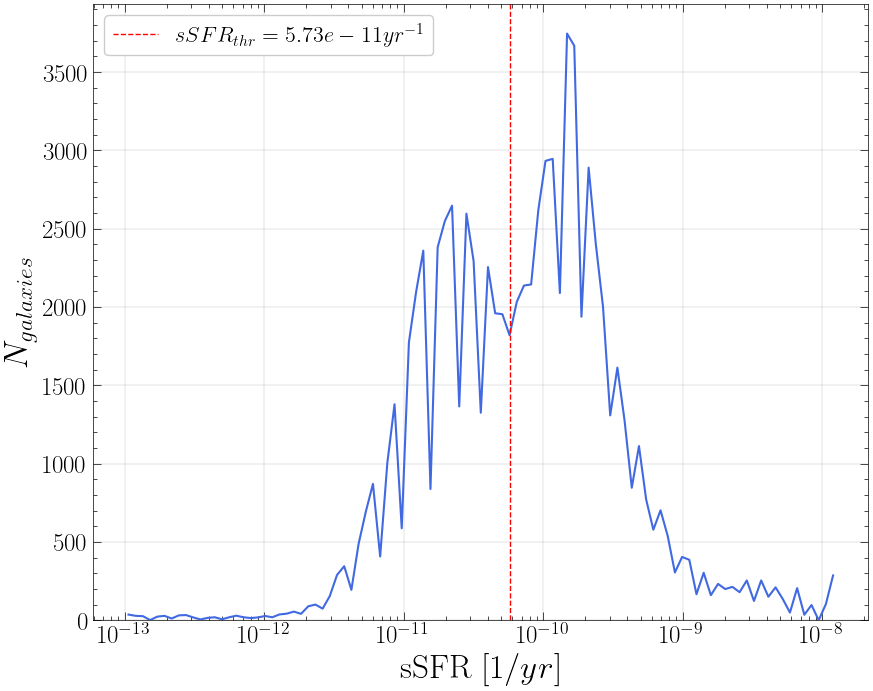
\includegraphics[width=\columnwidth]{images/marginalized_dist_mass.png}
	\caption{Marginalized distribution over the mass. The minimum between the two peaks corresponds to \(\mathrm{sSFR}_{\mathrm{thr}} = 10^{-10.24}\ \mathrm{yr^{-1}}\). This sets the threshold between the \acrlong{ms} and the passive region.}
	\label{fig:marinalized_dist_mass}
\end{figure}

\subsection{Stellar mass threshold}

As already mentioned, we need to determine the threshold in stellar mass for the transition from the Open-box to the Closed-box solution. To do this, we used \eqref{eq:m_star_vs_m_halo} combined with the cooling diagram from \citet[Figure 8.6]{Mo2010}. Figure \ref{fig:m_halo_vs_m_star} shows the inverse of \eqref{eq:m_star_vs_m_halo}. From the cooling diagram, the halo's mass range for effective cooling is roughly in the \([10^9, 10^{12}]\ \mathrm{M_{\sun}}\) interval. We adjusted the right end of the interval to match the end of the first branch of the curve in Figure \ref{fig:m_halo_vs_m_star}, and to obtain an upper stellar mass threshold close to the beginning of the galaxy-dense region in the passive population. This led us to choose \([10^9, 10^{11.6}]\ \mathrm{M_{\sun}}\) for the halo's mass interval, which corresponds, through \eqref{eq:m_star_vs_m_halo}, to \([10^{4.28}, 10^{10.15}]\ \mathrm{M_{\sun}}\) in stellar mass. Therefore, we chose the value of \(10^{10.15}\ \mathrm{M_{\sun}}\) in stellar mass for the transition between the two models.
\begin{figure}
	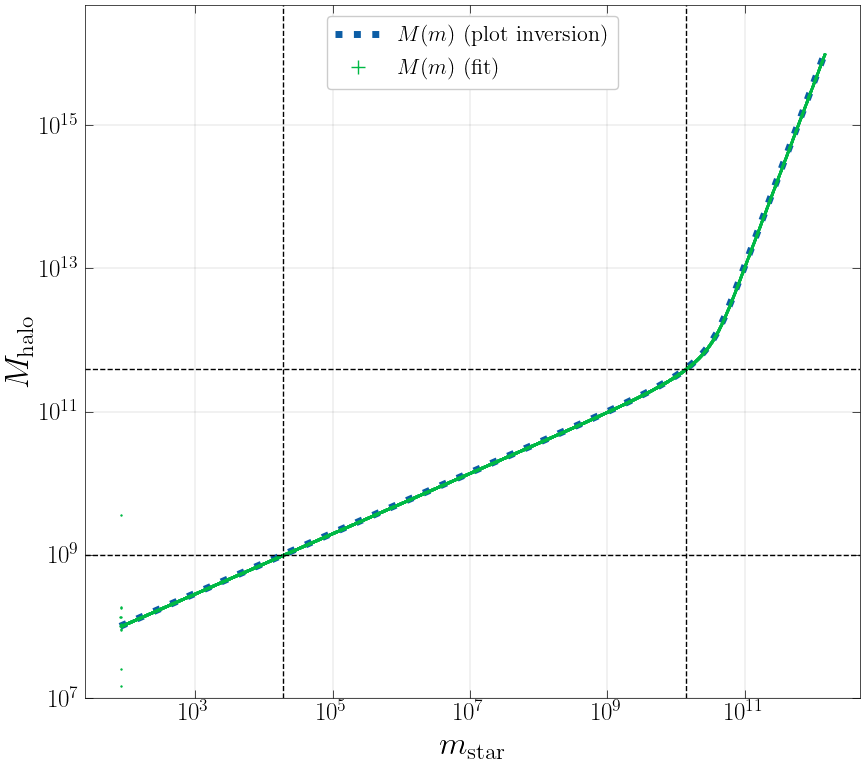
\includegraphics[width=\columnwidth]{images/m_halo_vs_m_star.png}
	\caption{Inverse of relation \eqref{eq:m_star_vs_m_halo} computed numerically. The dotted black lines mark the mass ranges for effective gas cooling on both axes. These are based on \citet[Figure 8.6]{Mo2010} with slight adjustment to match the beginning of the change in slope of the curve, and of the passive, galaxy-dense region in the \acrshort{ssfr} vs \(M_{\star}\) plane.}
	\label{fig:m_halo_vs_m_star}
\end{figure}

\subsection{Open-box solution}

Our Open-box model is controlled by two parameters: \(\eta\) and \(R\). The \(R\) parameter is constrained to the \([0, 1]\) interval and by our knowledge of stellar evolution processes. The \(\eta\) parameter is less constrained, and reasonable values should be of the order of unity. We tuned these parameters to match the curve of the model with the median of the \acrshort{ssfr} of the \acrshort{ms}. The result is shown in Figure \ref{fig:open_box_model} with the values of the parameters.
\begin{figure}
	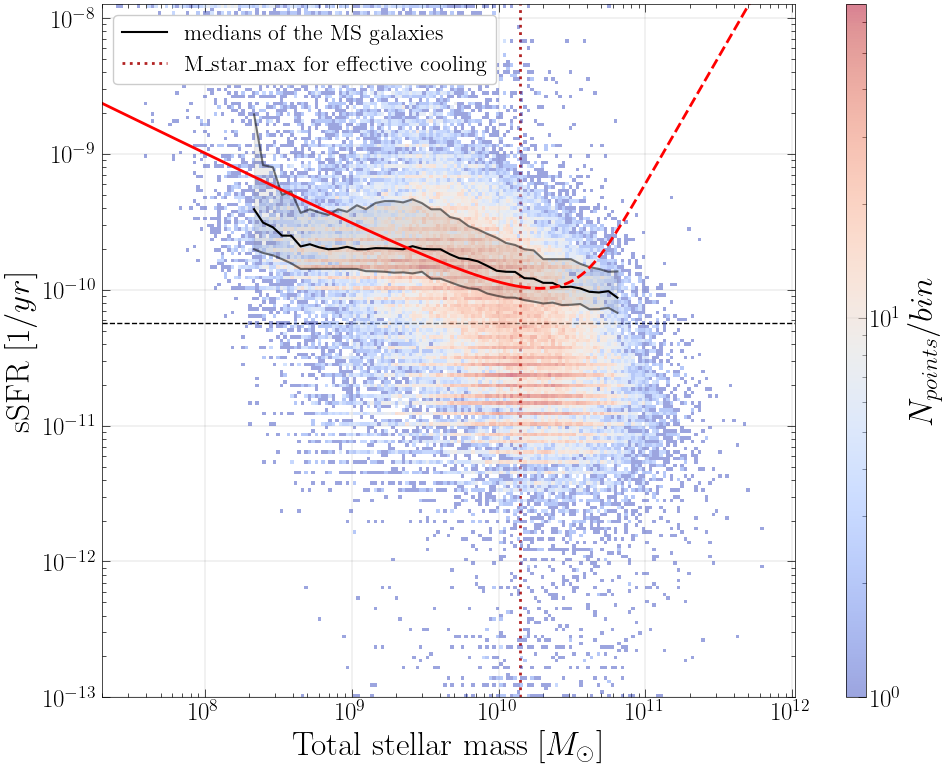
\includegraphics[width=\columnwidth]{images/open_box_model.png}
	\caption{Open-box model curve from \eqref{eq:open_box_solution}. The values of the model parameters are: \(\eta = 0.9\) and \(R = 0.4\). The horizontal dotted line represents the boundary between the \acrshort{ms} and the passive galaxies. The curve is dashed after the mass threshold for the transition between the Open-box and the Closed-box model.}
	\label{fig:open_box_model}
\end{figure}

\subsection{Adding the Closed-box solution}

Now we add the solution from the Closed-box model and match it with the Open-box at the boundary determined by the \(10^{10.15}\ \mathrm{M_{\sun}}\) vertical line. This model is controlled by five parameters: \(R\), \(\epsilon\), \(t_{\mathrm{dyn}}\), \(M_{\mathrm{gas}}(t_0)\), and \(M_{\star}(t_0)\). \(R\) is fixed to the same value used for the Open-box, and \(M_{\star}(t_0)\) (the stellar mass at the beginning of the Closed-box regime) is fixed at the boundary value of \(10^{10.15}\ \mathrm{M_{\sun}}\). \(M_{\mathrm{gas}}(t_0)\) is a free parameter we don't have any prior knowledge about; it shifts the model curve up and down, so we tuned it to match the Open-box curve at the boundary. Finally, \(\epsilon\) and \(t_{\mathrm{dyn}}\) control the slope of the curve, i.e., the speed of the depletion of the gas reservoir and the decline of the \acrshort{ssfr}. We tuned their values to achieve a good match with our data. The result is shown in Figure \ref{fig:combined_model}.
\begin{figure}
	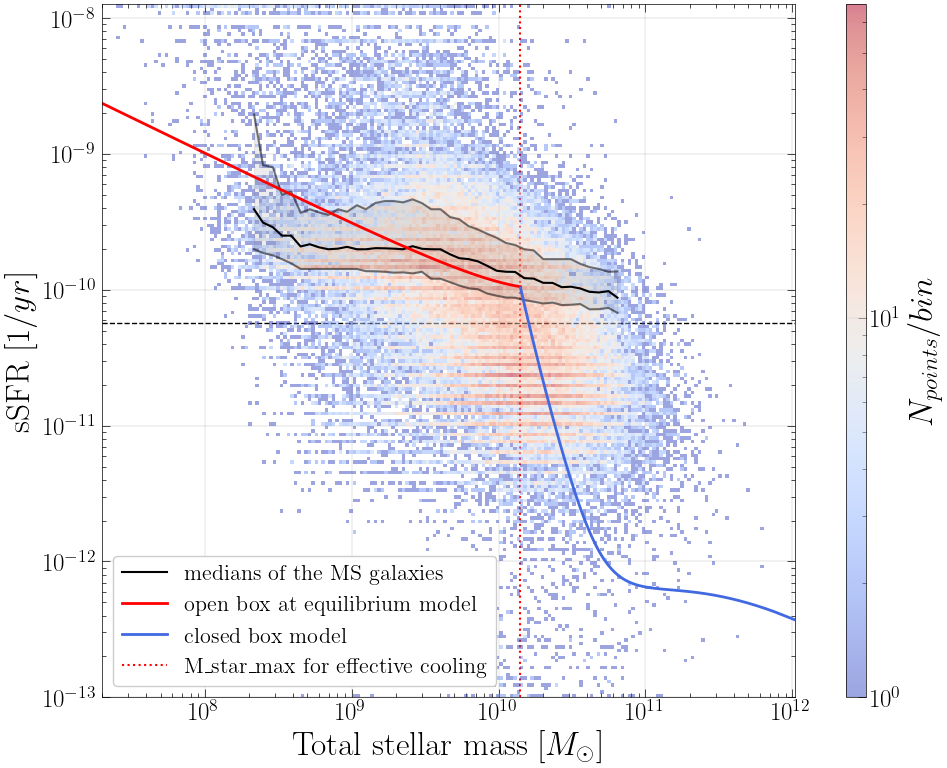
\includegraphics[width=\columnwidth]{images/combined_model.png}
	\caption{Combination of the Open-box \eqref{eq:open_box_solution} and the Closed-box \eqref{eq:closed_box_solution} models. The parameters are tuned to match the solutions at the boundary determined by the \(10^{10.15}\ \mathrm{M_{\sun}}\) stellar mass threshold. The Open-box parameters are the same as in Figure \ref{fig:open_box_model}. For the Closed-box, we have: \(R = 0.4\), \(\epsilon = 0.01\), \(t_{\mathrm{dyn}} = 2.7 \times 10^7\ \mathrm{yr}\), \(M_{\mathrm{gas}}(t_0) = 10^{9.75}\ \mathrm{M_{\sun}}\), and \(M_{\star}(t_0) = 10^{10.15}\ \mathrm{M_{\sun}}\).}
	\label{fig:combined_model}
\end{figure}

\subsection{Numerical model solutions}

As already mentioned, the numerical approach captures the shape of the data in the \acrshort{ssfr} vs \(M_{\star}\) plane, but not the correct magnitude of the \acrshort{ssfr}. For visualization purposes, the curves have been manually scaled to overlap with the data. In addition to the \(R\), \(\eta\), and \(\epsilon\) parameters already encountered, we also have the \([M_{\mathrm{H, min}}, M_{\mathrm{H, max}}]\) mass range for effective cooling explicitly coded in the Python script of the model. This mass range has been set to \([10^9, 10^{11.6}]\ \mathrm{M_{\sun}}\) as found before. We present the (scaled) results for two different implementations of the \(\xi\) function in Equation \ref{eq:gas_in}: the step function and the function from \citet[Figure 1]{Dave2011}, respectively in Figures \ref{fig:numerical_model_step} and \ref{fig:numerical_model_dave}. The net difference between the two is that the \citeauthor{Dave2011} implementation has a smoother transition in its functional form compared with the step function.
\begin{figure}
	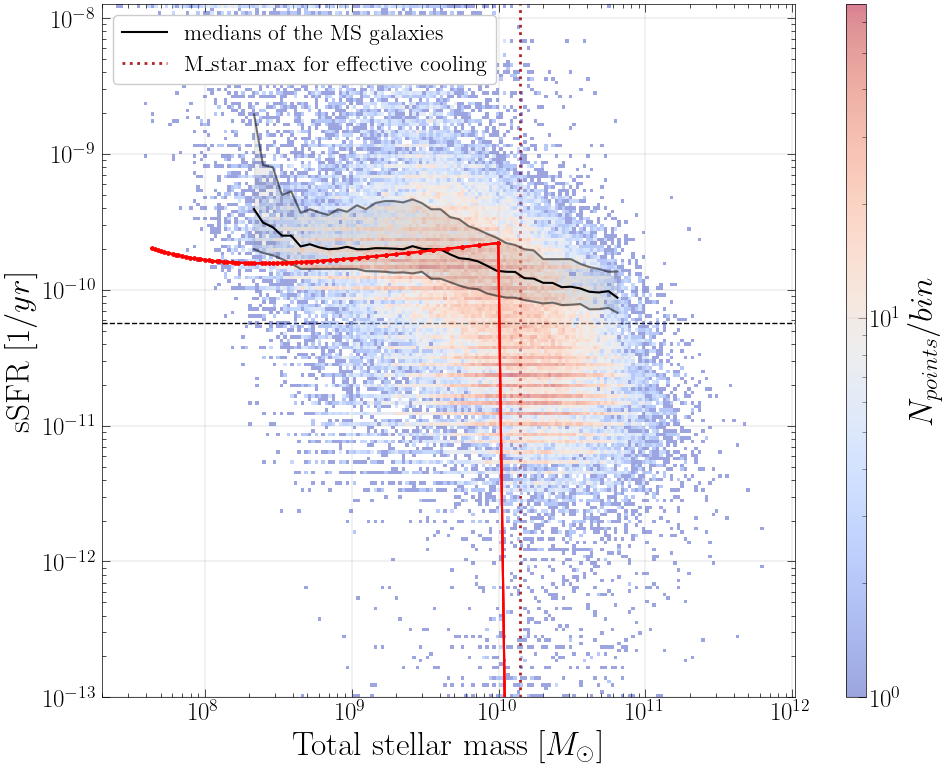
\includegraphics[width=\columnwidth]{images/numerical_model_step.png}
	\caption{Numerical model with a step function for \(\xi\) in Equation \ref{eq:gas_in}. Values of the parameters are: \(R = 0.1\), \(\epsilon = 0.02\), \(\eta = 4\). The curve is manually scaled by a factor of \(4\) for visualization purposes.}
	\label{fig:numerical_model_step}
\end{figure}
\begin{figure}
	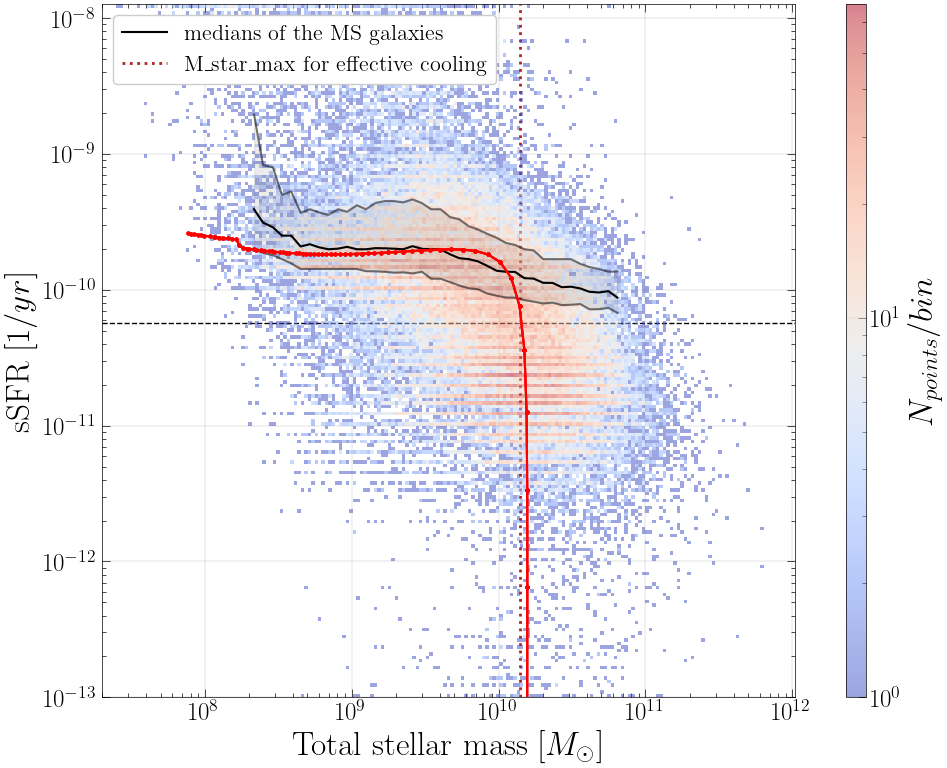
\includegraphics[width=\columnwidth]{images/numerical_model_dave.png}
	\caption{Numerical model with the \citet{Dave2011} implementation for \(\xi\) in Equation \ref{eq:gas_in}. Values of the parameters are: \(R = 0.4\), \(\epsilon = 0.02\), \(\eta = 1.3\). The curve is manually scaled by a factor of \(7\) for visualization purposes.}
	\label{fig:numerical_model_dave}
\end{figure}

\section{Discussion}

We believe that for \acrshort{ms} galaxies, the Open-box model (Figure \ref{fig:open_box_model}) is a fairly good representation of our data. The achievement of an equilibrium regime seems to be a good approximation for the majority of the \acrlong{ms}, but it isn't very reliable at the low mass end where the model diverges from the \acrshort{ssfr} median. This might be related mostly to the larger presence of younger galaxies in that mass range. Figure \ref{fig:ssfr_vs_mass_vs_age} shows the age distribution of galaxies in the two populations.
\begin{figure}
	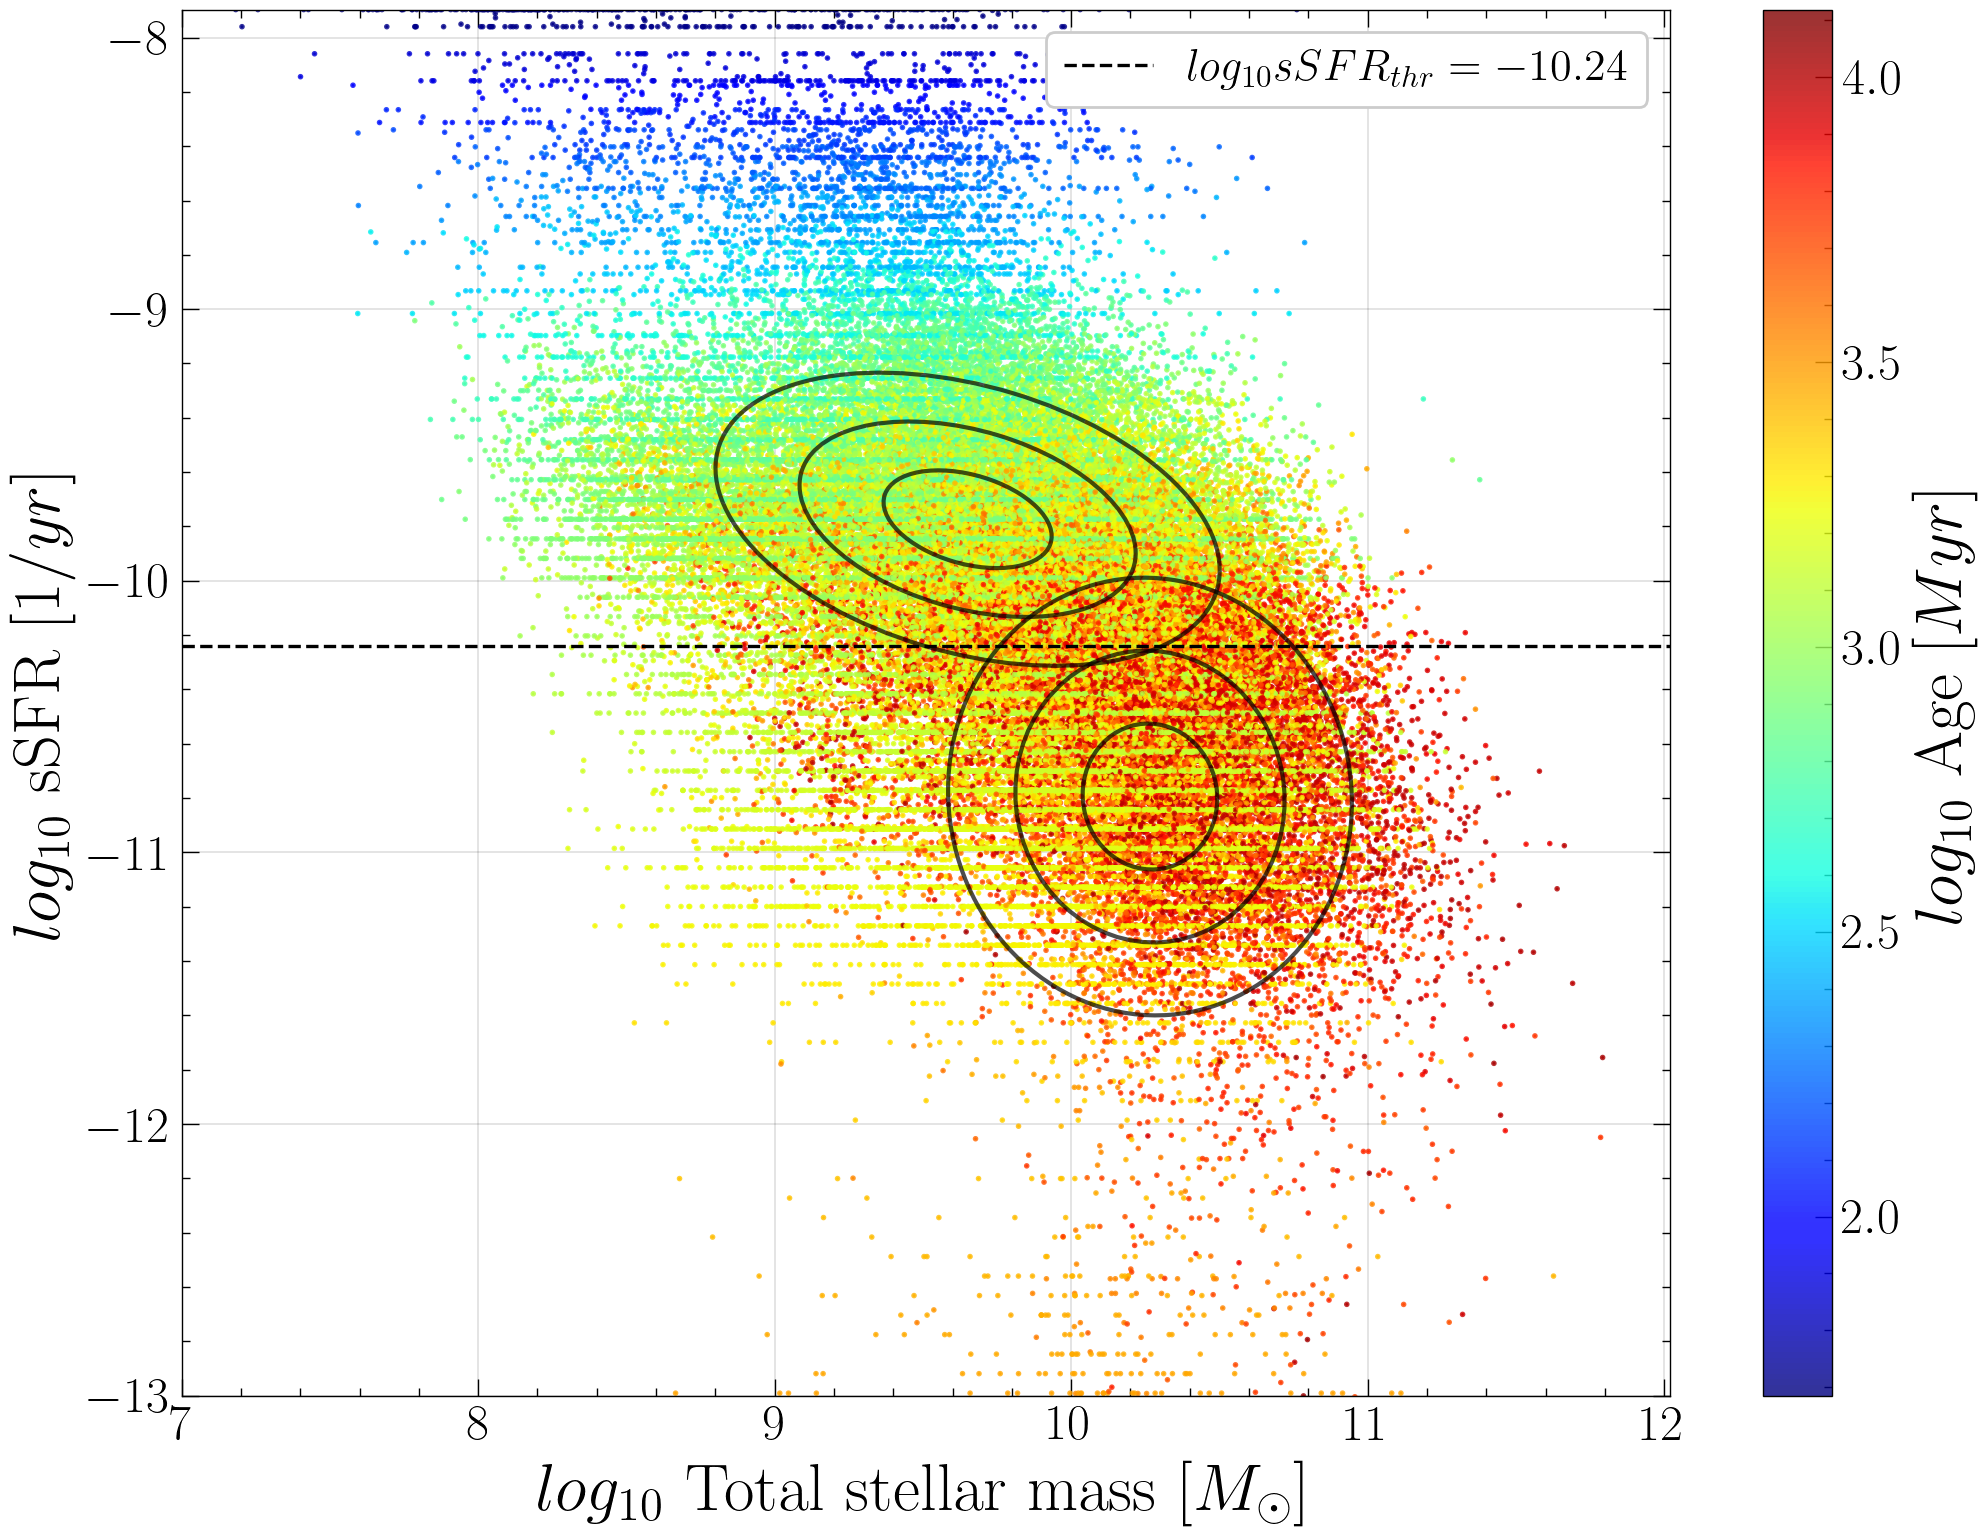
\includegraphics[width=\columnwidth]{images/sSFR_vs_mass_age_colormap.png}
	\caption{\acrshort{ssfr} vs \(M_{\star}\) diagram. Galaxies are colored based on their age. The two populations are depicted using contour levels of two bivariate normal distributions.}
	\label{fig:ssfr_vs_mass_vs_age}
\end{figure}
Such younger galaxies may still be in a transition phase or might not have accreted a massive enough \acrshort{dm} halo to effectively drive new gas into the galaxy. Indeed, this model doesn't consider the galaxy age and assumes that the gas reservoir has reached an equilibrium condition.

The Closed-box solution (blue line, Figure \ref{fig:combined_model}) roughly describes the declining trend of the \acrshort{ssfr}, and the mass threshold for the transition between the models is reasonable for our purposes. However the slope of the curve depends non-trivially on the values of \(R\), \(\epsilon\), \(t_{\mathrm{dyn}}\) and \(\dot{M}_{\mathrm{H}}\). This might be a source of degeneracy between those parameters for the optimal slope. Sometimes, models tuning led us to non-physical values of the parameters, maybe indicating that additional physical processes should be taken into account for a better description of both the \acrshort{ms} and the \acrshort{ssfr} quenching. Specifically, the Closed-box assumption for passive galaxies might be too strict for a meaningful description of the observations. Moreover, the results could benefit from a smoother transition between the two models similar to what has been done with the \citeauthor{Dave2011} \(\xi\) implementation. Is also worth noticing the discrepancy of the \(R\) and \(\eta\) values among the models in Figures \ref{fig:combined_model}, \ref{fig:numerical_model_step} and \ref{fig:numerical_model_dave}. In particular, the discrepancy between the numerical models and the time-independent one might be related to the fixed redshift approach of the latter, which doesn't consider that older galaxies had higher halo's accretion rates at high redshift, leading to higher halo masses and \(\eta\) values today.

Our numerical models present a noticeable discrepancy in magnitude from the data. However, the final shapes resemble the expected behavior. The simple implementation using a step function for \(\xi\) doesn't perform very well, leading to a too steep jump in the \acrshort{ssfr} in the passive region. Moreover, it doesn't fit our estimate for the transition between the two populations, starting its decline too early. On the other hand, the \citeauthor{Dave2011} \(\xi\) reproduces with more fidelity the slopes of the \acrshort{ms} and the passive galaxies, also respecting with good approximation our mass threshold for the transition. This also confirms that a sharp transition between the two \acrshort{sf} regimes is too simple an approximation for an accurate description of the two populations.

Regarding our initial questions:
\begin{enumerate}
	\item \textit{Can the two populations be described independently?} From our results, we think that the majority of the \acrshort{ms} can be described by an equilibrium model in which the variability of the \acrshort{ssfr} is mainly driven by the evolution of the \acrshort{dm} halo, as described by \eqref{eq:gas_in} and \eqref{eq:halo_accretion}. When the halo becomes too massive, the gas inflow in the galaxy declines rapidly due to ineffective gas cooling, leading to the observed quenching of the \acrshort{ssfr}. This behavior can be interpreted as a transition from an Open-box to a Closed-box model, even though our implementation is too simple to achieve a sufficient level of accuracy. In principle, the two populations could be described separately, but more complex models are needed.
	\item \textit{What determines the transition from the star-forming regime to the passive one?} The transition can be modeled considering the characteristic time scales of the virialized halo of the galaxy. If the cooling time is smaller than the dynamical time, galaxies can grow efficiently due to a consistent gas inflow. The growth of the halo changes the time scales, finally leading to a drop in the gas inflow and the consequent transition to the passive regime. A \(\xi\) function that comprehensively includes the physical processes acting during the transition plays a key role in the final results.
	\item \textit{Does redshift play a crucial role in the description of the two populations?} This might not be immediately evident from our fixed redshift approach, but correctly considering the age of the galaxies is crucial in the numerical models, in which galaxies are evolved from their formation up to the observation time. The constant halo accretion rate assumption made for the Closed-box model is probably too simple and should be avoided.
\end{enumerate}

Even though the Open-box solution performs well enough on the \acrshort{ms}, we believe that the numerical models could, in principle, fit better the two populations problem by encoding more precisely the ongoing physical processes. However, we couldn't address the wrong magnitude issue, probably indicating a misestimation of the gas inflow and outflow rates.

\section{Summary}

From galaxy observations, we can divide them into two populations: star-forming galaxies and passive galaxies. We found that the quenching of the \acrshort{ssfr} can be described by a time-evolving model of a galaxy starting with a fixed halo mass, by using the empirical relations for the halo's accretion rate \eqref{eq:halo_accretion} and the \acrlong{sfr} \eqref{eq:kennicutt}. Our solution doesn't capture the correct magnitude of the \acrshort{ssfr}, but this might be related to a misestimation of the gas inflow and outflow rates.

Using an empirical relation between the stellar mass and the halo mass \eqref{eq:m_star_vs_m_halo} and a cooling diagram for the halo's gas \citep[Figure 8.6]{Mo2010}, we could set a stellar mass threshold to estimate the boundary between the two \acrlong{sf} regimes at \(10^{10.15}\ \mathrm{M_{\sun}}\) in stellar mass. This has been used to merge together the Open-box and the Closed-box solutions, computed using a fixed redshift. The Open-box solution fits well enough the \acrshort{ms}, but the Closed-box model is too simple to accurately describe the passive population. In particular, the constant halo accretion rate assumption is probably too strict.

In order to successfully model the \acrlong{sfr} of galaxies, it is necessary to understand the correct balance between the terms in Equation \ref{eq:gas_conservation}. Our models might benefit from the inclusion of additional effects such as AGN feedback or ram pressure stripping, when supernovae of type II aren't enough to explain the observed data. However, we believe that correctly modeling the growing halo and the related gas cooling through the \(\xi\) function has a key role in giving the correct shape at the final results.

%%%%%%%%%%%%%%%%%%%% REFERENCES %%%%%%%%%%%%%%%%%%

\bibliographystyle{mnras}
\bibliography{bibfile}
\nocite{Bouche2010}

%%%%%%%%%%%%%%%%% APPENDICES %%%%%%%%%%%%%%%%%%%%%

\appendix

\section{\(M_{\star}\) vs. \(M_{\mathrm{H}}\) relation parameters} \label{appendix:m_star_vs_m_halo_parameters}

List of equations and values for \(N\), \(M_1\), \(\beta\) and \(\gamma\) in Equation \ref{eq:m_star_vs_m_halo} from \citet{Moster2012}.

\begin{align*}
	\log M_1(z) & = M_{10} + M_{11} \frac{z}{z + 1}           \\
	N(z)        & = N_{10} + N_{11} \frac{z}{z + 1}           \\
	\beta(z)    & = \beta_{10} + \beta_{11} \frac{z}{z + 1}   \\
	\gamma(z)   & = \gamma_{10} + \gamma_{11} \frac{z}{z + 1}
\end{align*}

\begin{table}
	\caption{Parameters values for Equation \ref{eq:m_star_vs_m_halo}.}
	\label{tab:m_star_vs_m_halo_parameters}
	\begin{tabular}{cccccccc}
		\hline
		\(M_{10}\) & \(M_{11}\) & \(N_{10}\) & \(N_{11}\) & \(\beta_{10}\) & \(\beta_{11}\) & \(\gamma_{10}\) & \(\gamma_{11}\) \\
		\hline
		11.590     & 1.195      & 0.0351     & -0.0247    & 1.376          & -0.826         & 0.608           & 0.329           \\
		\hline
	\end{tabular}
\end{table}

%%%%%%%%%%%%%%%%%%%%%%%%%%%%%%%%%%%%%%%%%%%%%%%%%%

\end{document}
